\section{Converged Graph Relational Optimization Framework}

\begin{figure}
    \centering
    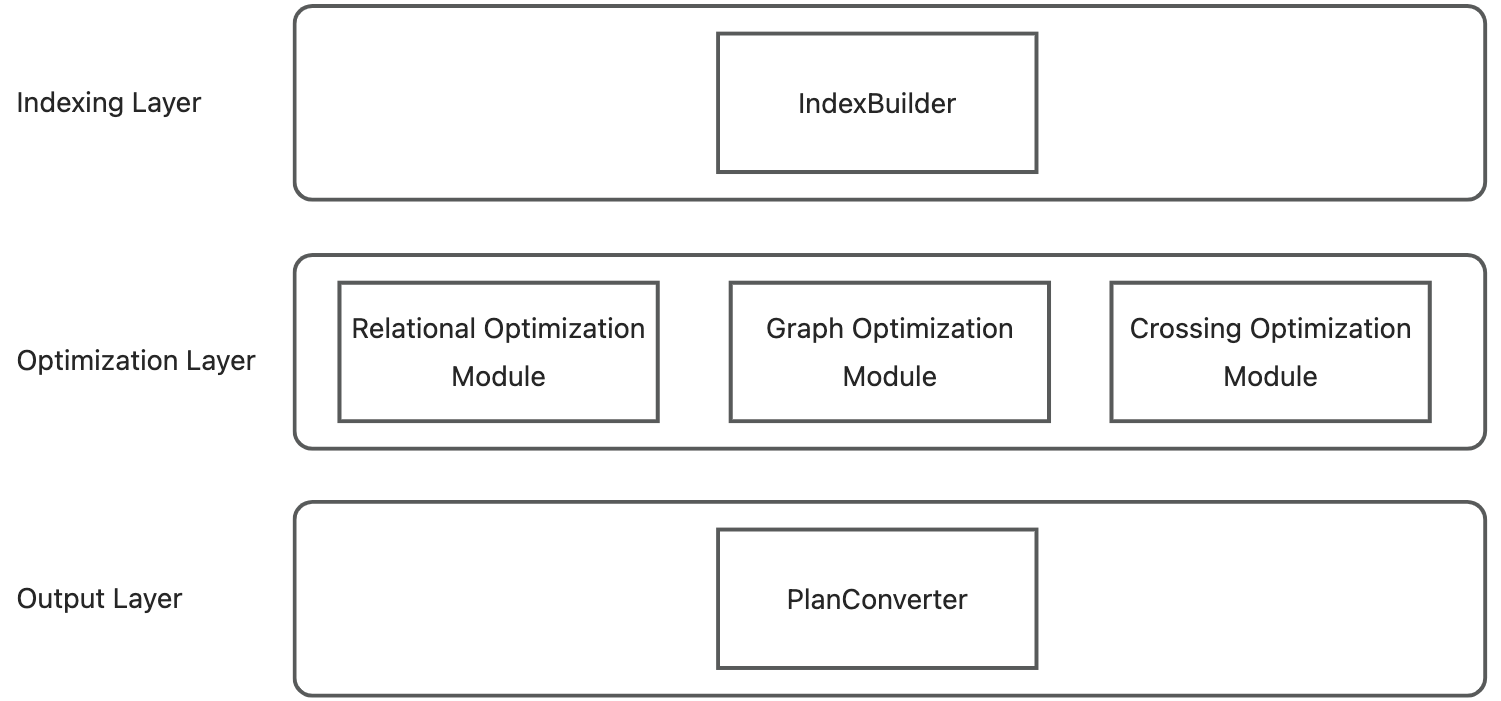
\includegraphics[width=\linewidth]{./figures/framework.png}
    \caption{Overview of the Converged Graph Relational Optimization Framwork.}
    \label{fig:framework-overview}
\end{figure}

\iffalse
\begin{corollary}
    There is an assumption that if a graph index is built on tables $vt_1, et_1, vt_2$, the vertices in $vt_1$ and $vt_2$ are stored in $V$, and the edges in $et_1$ are stored in $E$ of $\mathcal{M}(V, E, \mathcal{P})$.
\end{corollary}
\fi


To optimize SPJM queries efficiently, we propose the converged graph relational optimization framework.
The sketch of the converged graph relational optimization framework is shown in Fig.~\ref{fig:framework-overview}.

Specifically, given an SPJM query with several matching operators, the matching operators are first decomposed and the order of joins to obtain the pattern is optimized.
After graph matching decomposition, a logical plan is generated simultaneously, which is called the matching logical plan.
The operators that can be utilized in this plan include selection, projection, join, and matching operators.
Specifically, the matching operators should be minimum matching components.

Please note that the outputs of the matching logical plan is a graph relation, and after the selection $\widehat{\pi}$ is applied, a relational table $\widehat{R}$ is generated.
Then, the matching operator as well as $\widehat{\pi}$ are considered as a whole as an implementation of the scan operator (named ScanMatchTable), which is involved in the optimization of the other operators.
The implementation of ScanMatchTable is called the match scanning plan.
Since the matching operator is decomposed into a sequence of SPJ operators, the cardinality of the output of matching operator can be estimated, which is also the cardinality of ScanMatchTable.
After that, the left operators form an SPJ query (called the outer query), and the relational optimizers such as Calcite can be utilized to optimize the query.
The plan of the outer query is called the outer query plan.
Therefore, rich optimization strategies for relational databases can be applied.

In the process of optimization, graph matching decomposition and outer query are optimized by the match optimization module and relational optimization module, respectively.
Both rule-based optimizations and cost-based optimizations are utilized in these two modules.
For the relaional optimization module, we implement it with Calcite and propose two efficient rules specially for SPJM queries.
These rules push predicates in outer queries to matching operator to filter out the invalid elements early, and the details are introduced in Sec.~\ref{sec:optimizations}.
For the match optimization module, we implemement it with GLogS, which is one of the state-of-the-art graph optimizers.

As different databases usually support different operators and their physical plans can be greatly varied, it is of critical importance for an optimization framework to be flexible.
Therefore, we implement a PlanConverter in the framework to ensure the flexibility.
Given the generated optimal physical plan, the PlanConverter transforms the plan to an internal representation (e.g., Substrait \cite{substrait}), and then the internal representation is transformed to the physical plan that can be executed by the target database.
Finally, the plan is executed and the query results are obtained.
The above process of query processing is illustrated with the following example.


\begin{figure}
    \centering
    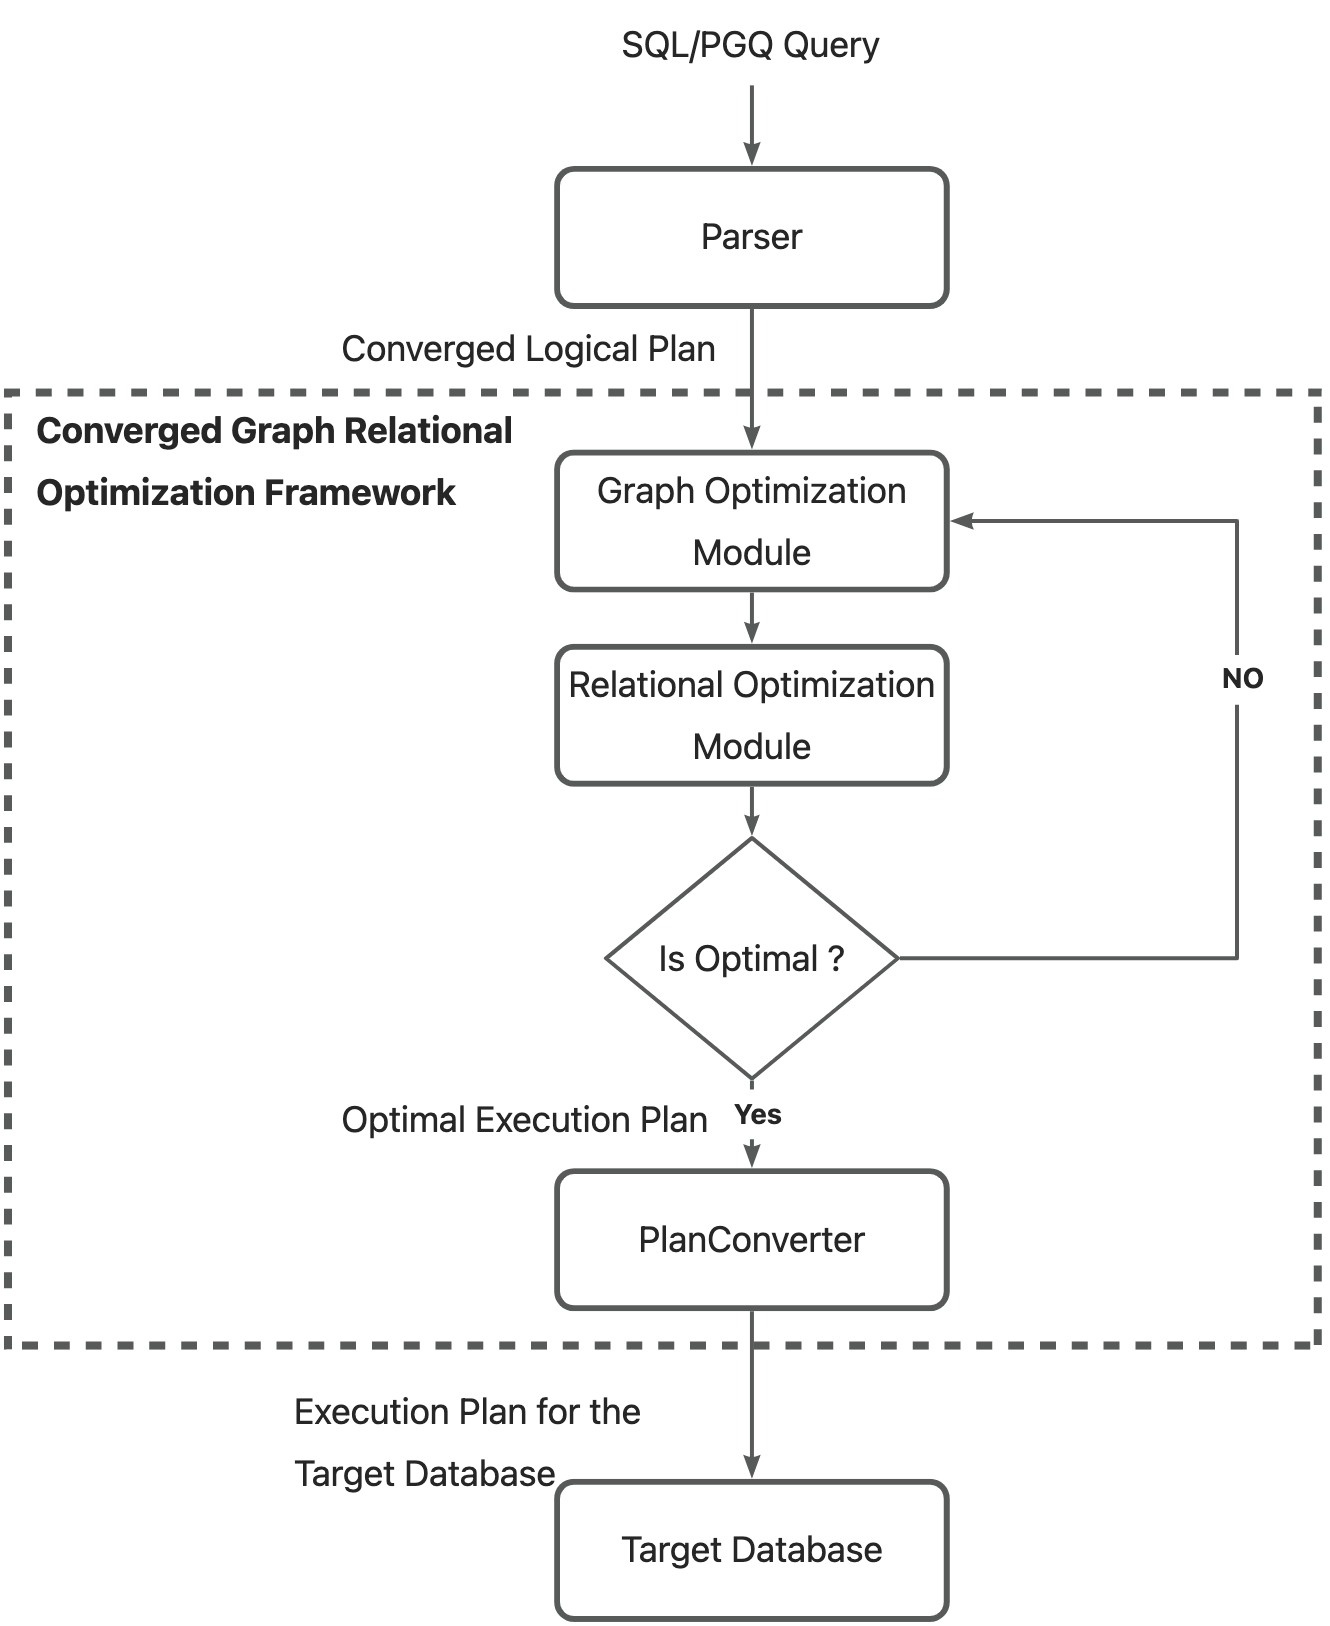
\includegraphics[width=.8\linewidth]{./figures/workflow.png}
    \caption{Workflow of the Converged Graph Relational Optimization Framework.}
    \label{fig:workflow}
\end{figure}

\begin{figure}
    \centering
    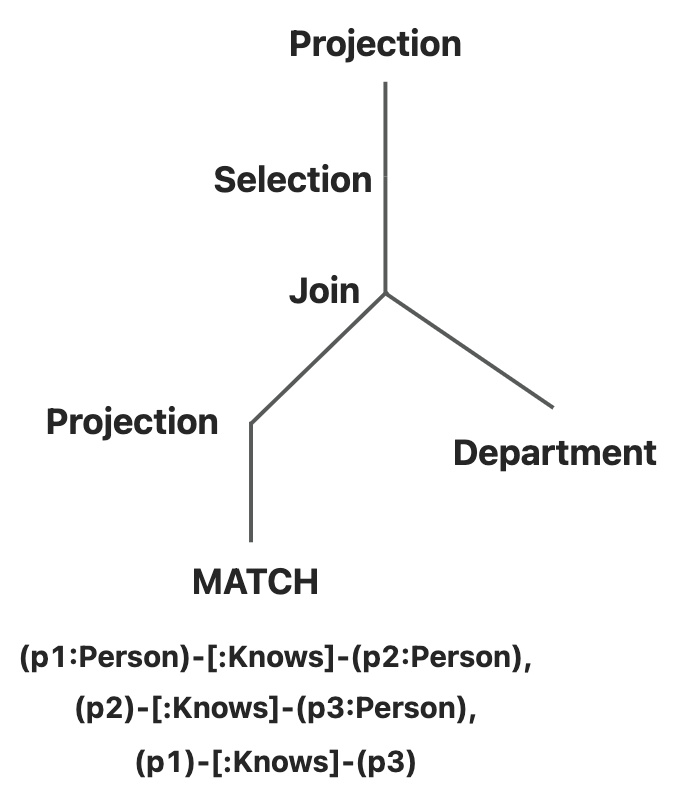
\includegraphics[width=.6\linewidth]{./figures/example_tree.png}
    \caption{The operator tree of SPJM query in Example \ref{example:framework}.}
    \label{fig:example-operator-tree}
\end{figure}

\begin{figure*}
    \centering
    \begin{subfigure}[b]{0.4\linewidth}
        \centering
        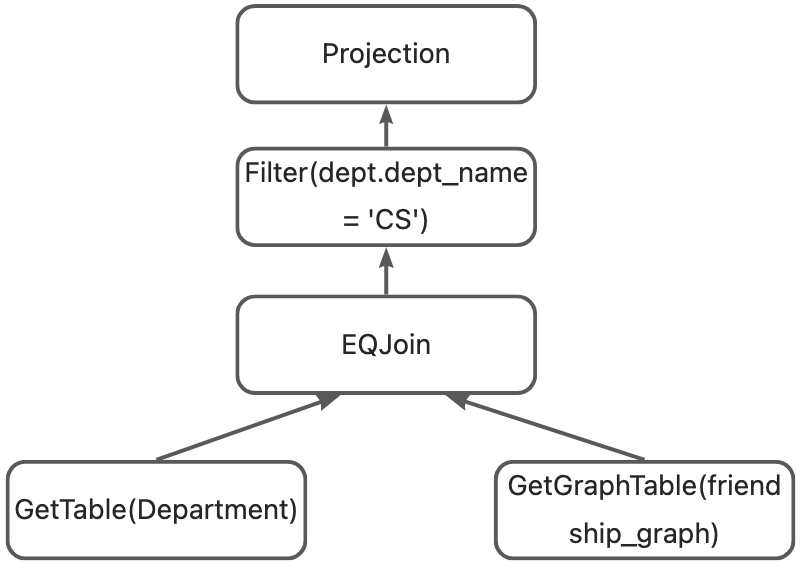
\includegraphics[width=\linewidth]{./figures/converged-logical-plan-relational.png}
        \caption{Outer query plan.}
        \label{fig:converged-logical-plan-relational}
    \end{subfigure}
    \begin{subfigure}[b]{0.4\linewidth}
        \centering
        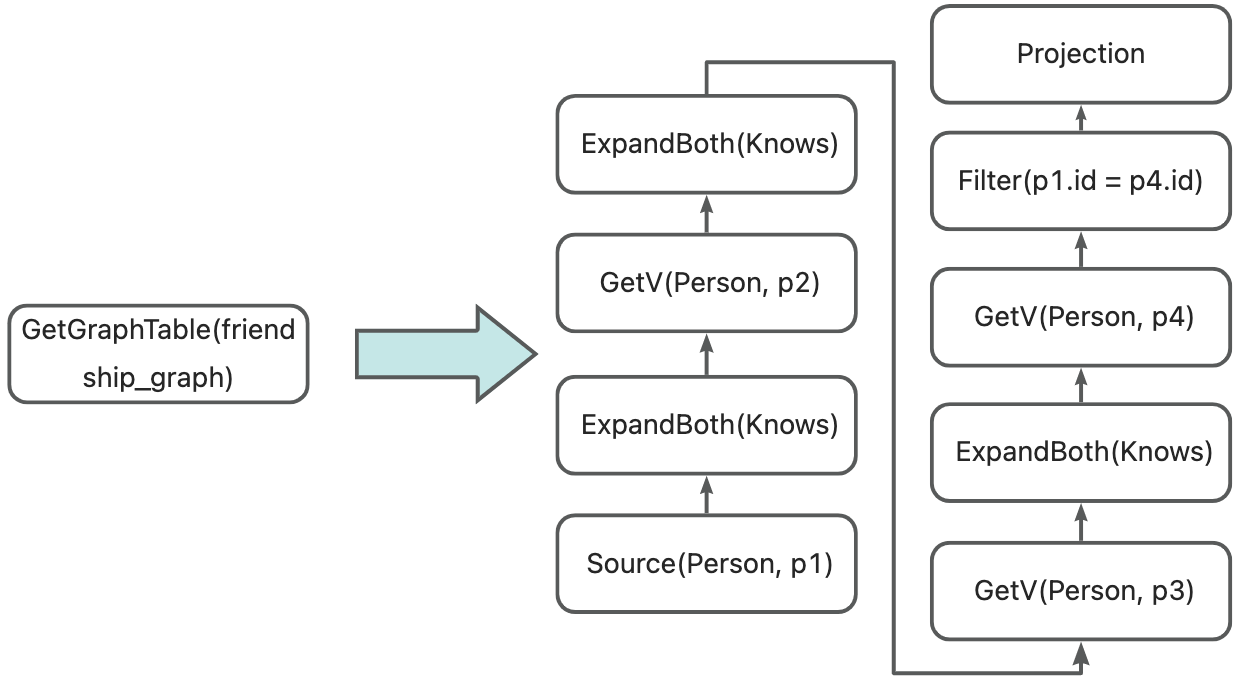
\includegraphics[width=\linewidth]{./figures/converged-logical-plan-graph.png}
        \caption{Match scanning plan.}
        \label{fig:converged-logical-plan-graph}
    \end{subfigure}
    \begin{subfigure}[b]{0.4\linewidth}
        \centering
        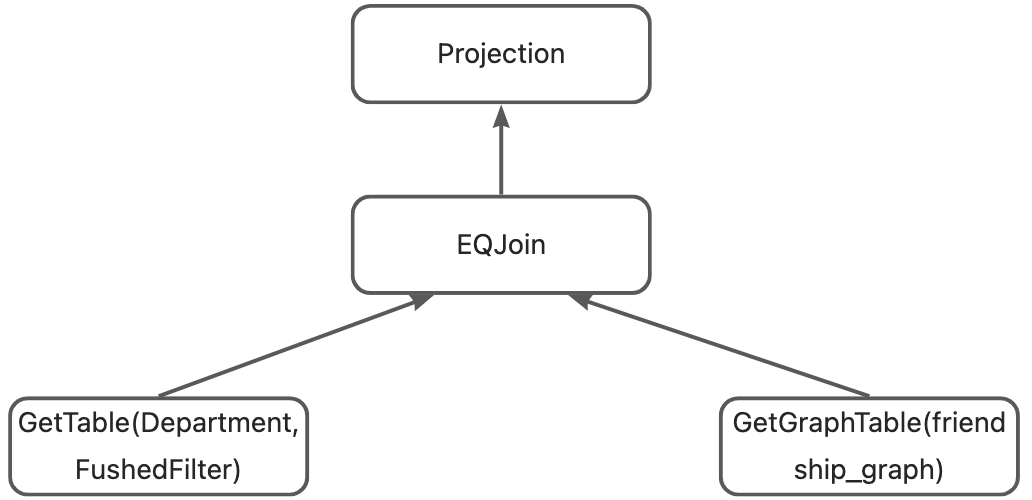
\includegraphics[width=\linewidth]{./figures/converged-logical-plan-relational-optimized.png}
        \caption{Outer query plan after Optimization.}
        \label{fig:relational-plan-optimized}
    \end{subfigure}
    \begin{subfigure}[b]{0.4\linewidth}
        \centering
        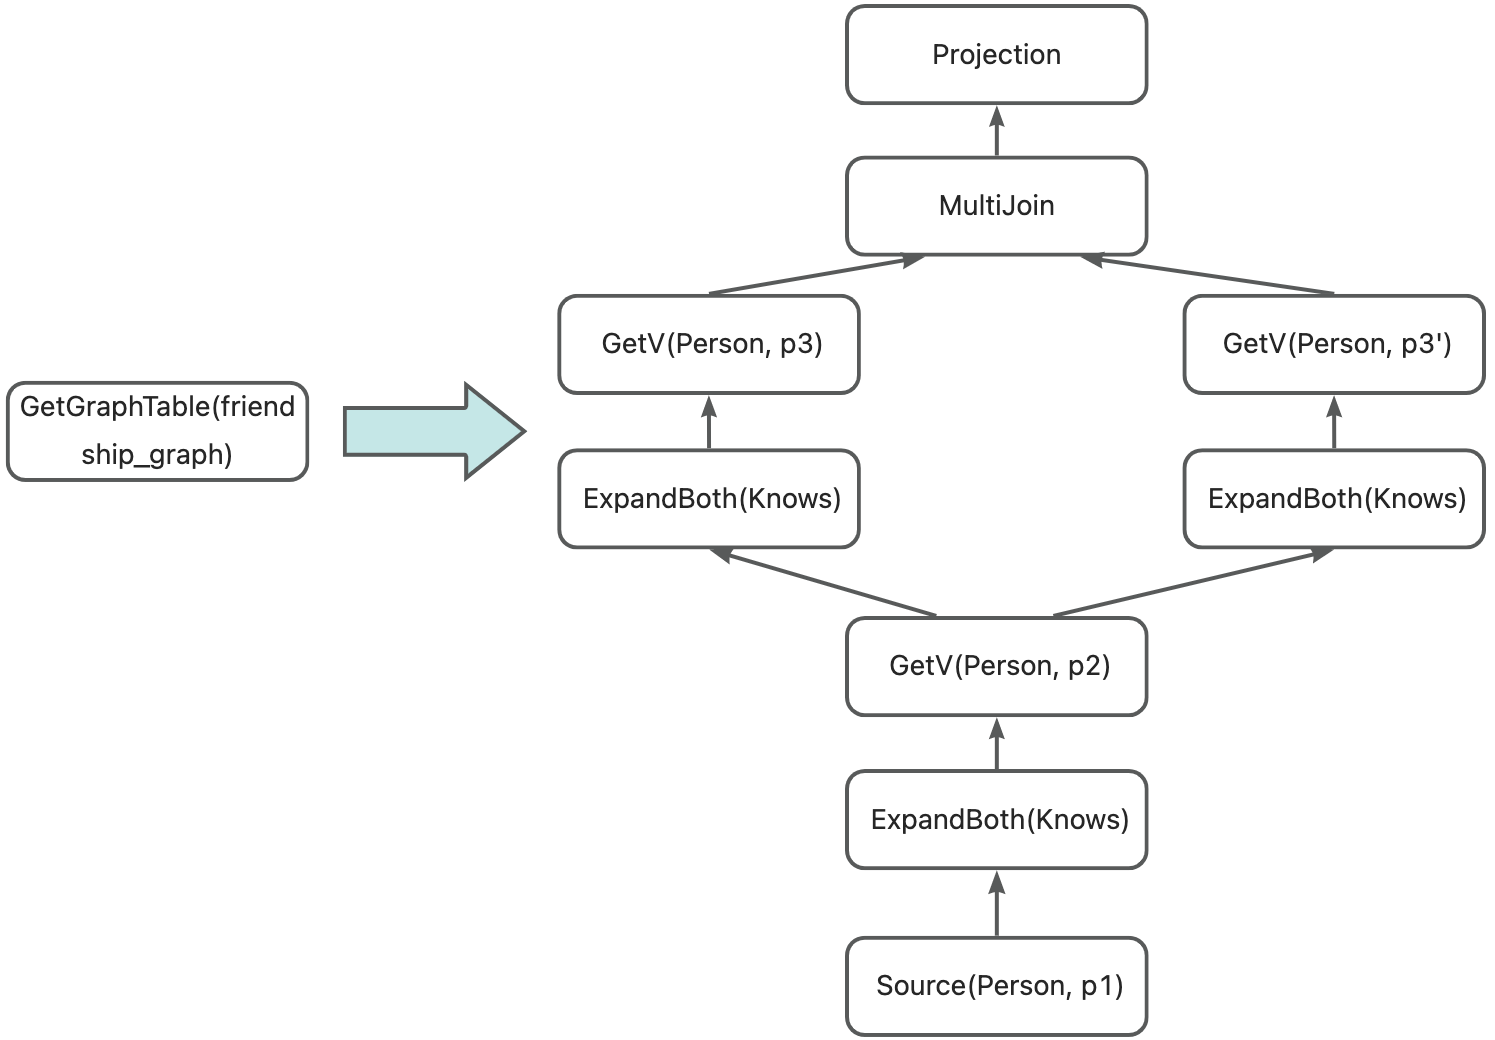
\includegraphics[width=\linewidth]{./figures/converged-logical-plan-graph-optimized.png}
        \caption{Match scanning plan after Optimization.}
        \label{fig:graph-plan-optimized}
    \end{subfigure}
    \begin{subfigure}[b]{0.5\linewidth}
        \centering
        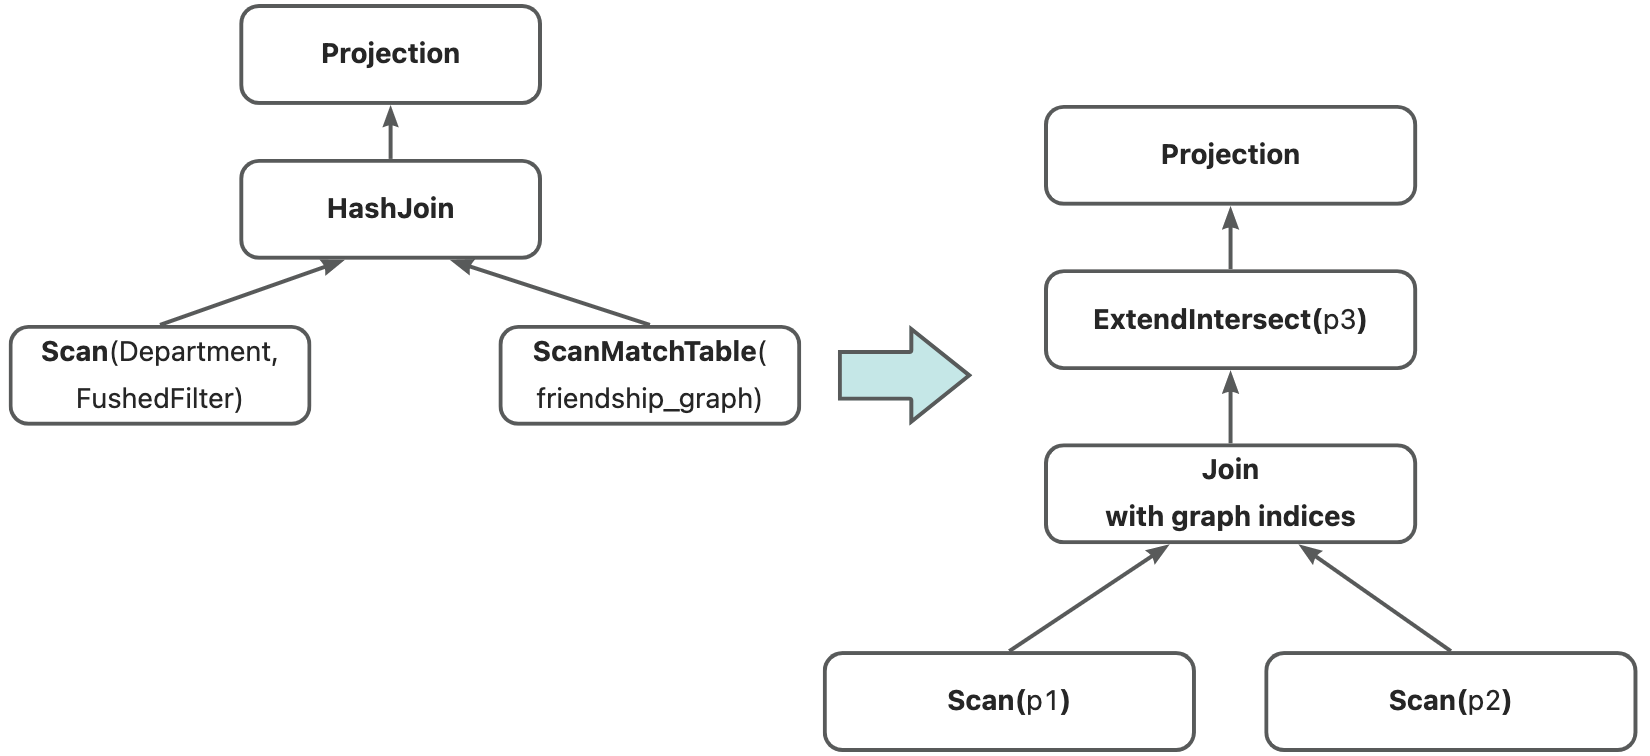
\includegraphics[width=\linewidth]{./figures/converged-physical-plan.png}
        \caption{Obtained Optimial Physical Plan.}
        \label{fig:physical-plan-optimized}
    \end{subfigure}
    \caption{An example of query opitmization.}
    \label{fig:query-grtree-example}
\end{figure*}



The above process of query processing is illustrated with the following example.

\begin{example}
    \label{example:framework}
    Given a relational database with tables as follows,
    \begin{equation*}
        \begin{split}
            & \textit{Person = (\underline{id}, name, dept\_id)} \\
            & \textit{Knows = (\underline{id1}, \underline{id2})} \\
            & \textit{Department = (\underline{dept\_id}, dept\_name)}, \\
        \end{split}
    \end{equation*}
    suppose we are going to find three persons satisfying: 
    (1) These three persons know each other;
    (2) At least two of them are from the department of computer science.
    The SPJM query can be illustrated as shown in Fig.~\ref{fig:example-operator-tree}.
    
    In relational matching algebra, the SPJM query can be expressed as follows:
    Firstly, to obtain the triangles, the pattern $\mathcal{P}_{\triangle}$ is
    \begin{lstlisting}
        (p1:Person)-[:Knows]-(p2:Person),
        (p2)-[:Knows]-(p3:Person),
        (p1)-[:Knows]-(p3)
    \end{lstlisting}
    Then, to get the relational table that records the three person and their departments, the algebra expression is 
    \begin{equation*}
        \begin{split}
            \widehat{R}_{graph} = & \pi_{p1.name\rightarrow pn1, p1.dept\_id \rightarrow dept1,p2.name\rightarrow pn2, p2.dept\_id \rightarrow dept2,} \\
            & _{p3.name\rightarrow pn3, p3.dept\_id \rightarrow dept3}(\mathcal{M}(GR, \mathcal{P}_{\triangle})),
        \end{split}
    \end{equation*}
    where $GR$ is a graph relation with only one tuple, and each attribute of the tuple is a vertex or an edge.
    The vertices correspond to rows in table Person and edges correspond to rows in table Knows.

    Finally, to obtain the triangles of persons with at least two persons from the department of computer science, the algebra expression is
    \begin{equation*}
        \begin{split}
        \pi_{pn1, pn2, pn3}
        (& \sigma_{dept.dept\_name = \text{`Computer Science'}}( \\ 
        & dept \Join_{dept1=dept.dept\_id \land dept2=dept.dept\_id} \widehat{R}_{graph})).
        \end{split}
    \end{equation*}

    Based on the above algebra expressions, the match scanning plan is shown in Fig.~\ref{fig:converged-logical-plan-graph} and the outer query plan is shown in Fig.~\ref{fig:converged-logical-plan-relational}.
    
    Then, optimization modules in the optimization layer are applied to optimize the plans.
    The optimized plans are shown in Fig.~\ref{fig:relational-plan-optimized} and Fig.~\ref{fig:graph-plan-optimized}.
    Moreover, the finally obtained optimal physical plan is shown in Fig.~\ref{fig:physical-plan-optimized}.
\end{example}

